% Options for packages loaded elsewhere
% Options for packages loaded elsewhere
\PassOptionsToPackage{unicode}{hyperref}
\PassOptionsToPackage{hyphens}{url}
%
\documentclass[
  ignorenonframetext,
  aspectratio=169,
]{beamer}
\newif\ifbibliography
\usepackage{pgfpages}
\setbeamertemplate{caption}[numbered]
\setbeamertemplate{caption label separator}{: }
\setbeamercolor{caption name}{fg=normal text.fg}
\beamertemplatenavigationsymbolsempty
% remove section numbering
\setbeamertemplate{part page}{
  \centering
  \begin{beamercolorbox}[sep=16pt,center]{part title}
    \usebeamerfont{part title}\insertpart\par
  \end{beamercolorbox}
}
\setbeamertemplate{section page}{
  \centering
  \begin{beamercolorbox}[sep=12pt,center]{section title}
    \usebeamerfont{section title}\insertsection\par
  \end{beamercolorbox}
}
\setbeamertemplate{subsection page}{
  \centering
  \begin{beamercolorbox}[sep=8pt,center]{subsection title}
    \usebeamerfont{subsection title}\insertsubsection\par
  \end{beamercolorbox}
}
% Prevent slide breaks in the middle of a paragraph
\widowpenalties 1 10000
\raggedbottom
\AtBeginPart{
  \frame{\partpage}
}
\AtBeginSection{
  \ifbibliography
  \else
    \frame{\sectionpage}
  \fi
}
\AtBeginSubsection{
  \frame{\subsectionpage}
}
\usepackage{iftex}
\ifPDFTeX
  \usepackage[T1]{fontenc}
  \usepackage[utf8]{inputenc}
  \usepackage{textcomp} % provide euro and other symbols
\else % if luatex or xetex
  \usepackage{unicode-math} % this also loads fontspec
  \defaultfontfeatures{Scale=MatchLowercase}
  \defaultfontfeatures[\rmfamily]{Ligatures=TeX,Scale=1}
\fi
\usepackage{lmodern}

\ifPDFTeX\else
  % xetex/luatex font selection
\fi
% Use upquote if available, for straight quotes in verbatim environments
\IfFileExists{upquote.sty}{\usepackage{upquote}}{}
\IfFileExists{microtype.sty}{% use microtype if available
  \usepackage[]{microtype}
  \UseMicrotypeSet[protrusion]{basicmath} % disable protrusion for tt fonts
}{}
\makeatletter
\@ifundefined{KOMAClassName}{% if non-KOMA class
  \IfFileExists{parskip.sty}{%
    \usepackage{parskip}
  }{% else
    \setlength{\parindent}{0pt}
    \setlength{\parskip}{6pt plus 2pt minus 1pt}}
}{% if KOMA class
  \KOMAoptions{parskip=half}}
\makeatother


\usepackage{longtable,booktabs,array}
\usepackage{calc} % for calculating minipage widths
\usepackage{caption}
% Make caption package work with longtable
\makeatletter
\def\fnum@table{\tablename~\thetable}
\makeatother
\usepackage{graphicx}
\makeatletter
\newsavebox\pandoc@box
\newcommand*\pandocbounded[1]{% scales image to fit in text height/width
  \sbox\pandoc@box{#1}%
  \Gscale@div\@tempa{\textheight}{\dimexpr\ht\pandoc@box+\dp\pandoc@box\relax}%
  \Gscale@div\@tempb{\linewidth}{\wd\pandoc@box}%
  \ifdim\@tempb\p@<\@tempa\p@\let\@tempa\@tempb\fi% select the smaller of both
  \ifdim\@tempa\p@<\p@\scalebox{\@tempa}{\usebox\pandoc@box}%
  \else\usebox{\pandoc@box}%
  \fi%
}
% Set default figure placement to htbp
\def\fps@figure{htbp}
\makeatother





\setlength{\emergencystretch}{3em} % prevent overfull lines

\providecommand{\tightlist}{%
  \setlength{\itemsep}{0pt}\setlength{\parskip}{0pt}}



 


\makeatletter
\@ifpackageloaded{tcolorbox}{}{\usepackage[skins,breakable]{tcolorbox}}
\@ifpackageloaded{fontawesome5}{}{\usepackage{fontawesome5}}
\definecolor{quarto-callout-color}{HTML}{909090}
\definecolor{quarto-callout-note-color}{HTML}{0758E5}
\definecolor{quarto-callout-important-color}{HTML}{CC1914}
\definecolor{quarto-callout-warning-color}{HTML}{EB9113}
\definecolor{quarto-callout-tip-color}{HTML}{00A047}
\definecolor{quarto-callout-caution-color}{HTML}{FC5300}
\definecolor{quarto-callout-color-frame}{HTML}{acacac}
\definecolor{quarto-callout-note-color-frame}{HTML}{4582ec}
\definecolor{quarto-callout-important-color-frame}{HTML}{d9534f}
\definecolor{quarto-callout-warning-color-frame}{HTML}{f0ad4e}
\definecolor{quarto-callout-tip-color-frame}{HTML}{02b875}
\definecolor{quarto-callout-caution-color-frame}{HTML}{fd7e14}
\makeatother
\makeatletter
\@ifpackageloaded{caption}{}{\usepackage{caption}}
\AtBeginDocument{%
\ifdefined\contentsname
  \renewcommand*\contentsname{Table of contents}
\else
  \newcommand\contentsname{Table of contents}
\fi
\ifdefined\listfigurename
  \renewcommand*\listfigurename{List of Figures}
\else
  \newcommand\listfigurename{List of Figures}
\fi
\ifdefined\listtablename
  \renewcommand*\listtablename{List of Tables}
\else
  \newcommand\listtablename{List of Tables}
\fi
\ifdefined\figurename
  \renewcommand*\figurename{Figure}
\else
  \newcommand\figurename{Figure}
\fi
\ifdefined\tablename
  \renewcommand*\tablename{Table}
\else
  \newcommand\tablename{Table}
\fi
}
\@ifpackageloaded{float}{}{\usepackage{float}}
\floatstyle{ruled}
\@ifundefined{c@chapter}{\newfloat{codelisting}{h}{lop}}{\newfloat{codelisting}{h}{lop}[chapter]}
\floatname{codelisting}{Listing}
\newcommand*\listoflistings{\listof{codelisting}{List of Listings}}
\makeatother
\makeatletter
\makeatother
\makeatletter
\@ifpackageloaded{caption}{}{\usepackage{caption}}
\@ifpackageloaded{subcaption}{}{\usepackage{subcaption}}
\makeatother

\usepackage{bookmark}
\IfFileExists{xurl.sty}{\usepackage{xurl}}{} % add URL line breaks if available
\urlstyle{same}
\hypersetup{
  pdftitle={Análise Fatorial},
  hidelinks,
  pdfcreator={LaTeX via pandoc}}



\title{Análise Fatorial}
\author{}
\date{}

\begin{document}
\frame{\titlepage}


\begin{frame}{Análise Fatorial}
\phantomsection\label{anuxe1lise-fatorial}
\begin{itemize}
\tightlist
\item
  \textbf{Objetivo:} Descrever as relações de covariância entre muitas
  variáveis em termos de poucas quantidades aleatórias subjacentes e não
  observáveis
\end{itemize}

\pause

\begin{itemize}
\tightlist
\item
  \textbf{Motivação:} Variáveis de um grupo altamente correlacionadas
  entre si, mas com pequenas correlações de outros grupos.

  \begin{itemize}
  \tightlist
  \item
    É concebível que cada grupo de variáveis represente um fator (ou
    construto) que seja o responsável pelas correlações observadas
  \end{itemize}
\end{itemize}
\end{frame}

\begin{frame}{Análise Fatorial}
\phantomsection\label{anuxe1lise-fatorial-1}
Vamos supor cinco variáveis \(Y_1\), \(Y_2\), \(Y_3\), \(Y_4\) e \(Y_5\)
correspondentes às notas de estudantes em Espanhol, Inglês, Química,
Física e Matemática, respectivamente.

\begin{longtable}[]{@{}cccccc@{}}
\caption{Matriz de correlações
hipotética}\label{tbl-correlacao}\tabularnewline
\toprule\noalign{}
& \(Y_1\) & \(Y_2\) & \(Y_3\) & \(Y_4\) & \(Y_5\) \\
\midrule\noalign{}
\endfirsthead
\toprule\noalign{}
& \(Y_1\) & \(Y_2\) & \(Y_3\) & \(Y_4\) & \(Y_5\) \\
\midrule\noalign{}
\endhead
\(Y_1\) & 1 & 0,90 & 0,05 & 0,05 & 0,10 \\
\(Y_2\) & 0,90 & 1 & 0,05 & 0,10 & 0,05 \\
\(Y_3\) & 0,05 & 0,05 & 1 & 0,95 & 0,85 \\
\(Y_4\) & 0,05 & 0,10 & 0,95 & 1 & 0,90 \\
\(Y_5\) & 0,10 & 0,05 & 0,85 & 0,90 & 1 \\
\bottomrule\noalign{}
\end{longtable}
\end{frame}

\begin{frame}{Análise Fatorial}
\phantomsection\label{anuxe1lise-fatorial-2}
Com base nas correlações, poderíamos imaginar dois fatores subjacentes,
e não observáveis:

\begin{itemize}
\tightlist
\item
  \textbf{Fator 1:} Conhecimento em línguas - associado aos desempenhos
  em Espanhol e Inglês, fortemente correlacionados;
\end{itemize}

\pause

\begin{itemize}
\tightlist
\item
  \textbf{Fator 2:} Conhecimento em ciências exatas - associado aos
  desempenhos em Química, Física e Matemática.
\end{itemize}

\pause

É importante compreender que ``conhecimento'' é algo que não se mede
diretamente, mas que pode se manifestar através de variáveis
observáveis, como as notas obtidas nos exames.
\end{frame}

\begin{frame}{Análise Fatorial}
\phantomsection\label{anuxe1lise-fatorial-3}
Pode ser considerada uma extensão da Análise de Componentes Principais

\pause

\begin{itemize}
\tightlist
\item
  Ambas são tentativas de aproximar \(\boldsymbol{S}\).
\end{itemize}

\pause

\begin{itemize}
\tightlist
\item
  A aproximação baseada em Análise Fatorial é mais elaborada
\end{itemize}

\pause

Questão principal:

\begin{itemize}
\tightlist
\item
  Dados são consistentes com a estrutura prescrita?
\end{itemize}
\end{frame}

\begin{frame}{Tipos de Análise Fatorial}
\phantomsection\label{tipos-de-anuxe1lise-fatorial}
\begin{block}{Análise Fatorial Exploratória}
\phantomsection\label{anuxe1lise-fatorial-exploratuxf3ria}
\medskip

\begin{itemize}
\item
  Busca encontrar os fatores subjacentes às variáveis originais
  amostradas
\item
  Em geral, efetuada quando não se tem noção clara da quantidade de
  fatores do modelo e nem do que representam
\end{itemize}
\end{block}

\begin{block}{Análise Fatorial Confirmatória}
\phantomsection\label{anuxe1lise-fatorial-confirmatuxf3ria}
\begin{itemize}
\tightlist
\item
  Tem-se em mãos um modelo fatorial pré-especificado (modelo hipotético)
  e deseja-se verificar se é aplicável ou consistente com os dados
  amostrais de que dispõe
\end{itemize}
\end{block}
\end{frame}

\begin{frame}{Planejamento de uma análise fatorial}
\phantomsection\label{planejamento-de-uma-anuxe1lise-fatorial}
\begin{itemize}
\tightlist
\item
  \textbf{Verificar a adequabilidade da base de dados:} tamanho da
  amostra (desejável a razão de 5 indivíduos para cada variável),
  correlações significativas, KMO adequado.
\end{itemize}

\pause

\begin{itemize}
\tightlist
\item
  \textbf{Determinar o método de extração e o número de fatores a serem
  extraídos:} métodos de extração (componentes principais, fatores
  principais, máxima verossimilhança), número de fatores (critério de
  kaiser, screeplot, variância acumulada).
\end{itemize}

\pause

\begin{itemize}
\tightlist
\item
  \textbf{Decidir o tipo de rotação:} Varimax, Quartimax,
  Orthomax\ldots{}
\end{itemize}
\end{frame}

\begin{frame}{Planejamento de uma análise fatorial}
\phantomsection\label{planejamento-de-uma-anuxe1lise-fatorial-1}
\begin{block}{GIGO: Garbage In, Garbage Out!}
\phantomsection\label{gigo-garbage-in-garbage-out}
\begin{tcolorbox}[enhanced jigsaw, leftrule=.75mm, toprule=.15mm, colframe=quarto-callout-warning-color-frame, colbacktitle=quarto-callout-warning-color!10!white, breakable, toptitle=1mm, colback=white, rightrule=.15mm, title=\textcolor{quarto-callout-warning-color}{\faExclamationTriangle}\hspace{0.5em}{Cuidado!}, opacitybacktitle=0.6, coltitle=black, bottomtitle=1mm, titlerule=0mm, arc=.35mm, left=2mm, bottomrule=.15mm, opacityback=0]

\begin{itemize}
\tightlist
\item
  A análise fatorial sempre produzirá fatores. Desta forma, ela é sempre
  um candidato para o fenômeno \textbf{``lixo dentro, lixo fora''}.
\end{itemize}

\medskip

\begin{itemize}
\tightlist
\item
  Se o pesquisador incluir indiscriminadamente um grande número de
  variáveis e esperar que a análise fatorial ``faça revelações'', a
  possibilidade de resultados pobres será alta.
\end{itemize}

\medskip

\begin{itemize}
\tightlist
\item
  A qualidade e o significado dos fatores determinados refletem
  \textbf{estruturas conceituais} das variáveis incluídas na análise
  (base conceitual).
\end{itemize}

\end{tcolorbox}
\end{block}
\end{frame}

\begin{frame}{Planejamento de uma análise fatorial}
\phantomsection\label{planejamento-de-uma-anuxe1lise-fatorial-2}
\begin{block}{Questões conceituais\ldots{}}
\phantomsection\label{questuxf5es-conceituais}
\bigskip

\begin{itemize}
\tightlist
\item
  É responsabilidade do pesquisador garantir que os padrões observados
  sejam conceitualmente válidos. A AF é capaz somente de determinar a
  adequação das correlações entre variáveis.
\end{itemize}

\medskip

\begin{itemize}
\tightlist
\item
  O pesquisador deve garantir que a amostra esteja adequada à estrutura
  fatorial inerente.
\end{itemize}

\medskip

\begin{itemize}
\tightlist
\item
  Por exemplo, ao avaliar os fatores de risco de uma acidente vascular,
  se nenhuma variável relacionada aos fatores genéticos for incluída, a
  AF não será capaz de identificar esta dimensão.
\end{itemize}
\end{block}
\end{frame}

\begin{frame}{Planejamento de uma análise fatorial}
\phantomsection\label{planejamento-de-uma-anuxe1lise-fatorial-3}
\begin{block}{Questões conceituais\ldots{}}
\phantomsection\label{questuxf5es-conceituais-1}
\begin{itemize}
\tightlist
\item
  A qualidade e o significado dos fatores obtidos refletem as bases
  conceituais das variáveis incluídas na análise.
\end{itemize}

\medskip

\begin{itemize}
\tightlist
\item
  O pesquisador não deve incluir indiscriminadamente inúmeras variáveis
  e esperar que a AF ``arrume as coisas''.
\end{itemize}

\medskip

\begin{itemize}
\tightlist
\item
  No exemplo da avaliação dos fatores de risco de uma acidente vascular,
  incluir a variável, por exemplo, ``cor dos olhos'' interfere nos
  resultados da AF e não traz nenhuma informação relevante para o objeto
  de estudo.
\end{itemize}
\end{block}
\end{frame}

\begin{frame}{Planejamento de uma análise fatorial}
\phantomsection\label{planejamento-de-uma-anuxe1lise-fatorial-4}
\begin{block}{Questões estatísticas\ldots{}}
\phantomsection\label{questuxf5es-estatuxedsticas}
\begin{itemize}
\tightlist
\item
  Espera-se que haja correlações significativas, pois o objetivo é
  identificar conjuntos de variáveis inter-relacionadas.
\end{itemize}

\vspace{0.3cm}

\begin{itemize}
\tightlist
\item
  Se todas as correlações são pequenas ou iguais, o pesquisador deve
  questionar o uso da análise fatorial.
\end{itemize}

\vspace{0.3cm}

\begin{itemize}
\tightlist
\item
  Inspeção visual da matriz de correlação -- coeficientes pelo menos em
  torno de 0,30.
\end{itemize}
\end{block}
\end{frame}

\begin{frame}{Planejamento de uma análise fatorial}
\phantomsection\label{planejamento-de-uma-anuxe1lise-fatorial-5}
\begin{itemize}
\tightlist
\item
  \textbf{Teste de esfericidade de Bartlett (BTS):} O teste de
  esfericidade de Bartlett testa a hipótese de que as variáveis não
  sejam correlacionadas na população.
\end{itemize}

\[H_0: \boldsymbol{P} = \boldsymbol{I}\]

A estatística do teste é dada por

\[\chi^2 = -\left[ (n-1)-\dfrac{2p + 5}{6}\right] \ln|\boldsymbol{R}|\]

que tem uma distribuição qui-quadrado com \(\nu\) graus de liberdade,
sendo \(\nu = \dfrac{p(p-1)}{2}\), \(n\) igual ao tamanho da amostra,
\(p\) igual ao número de variáveis e \(|\boldsymbol{R}|\), o
determinante da matriz de correlação amostral.
\end{frame}

\begin{frame}{Planejamento de uma análise fatorial}
\phantomsection\label{planejamento-de-uma-anuxe1lise-fatorial-6}
\begin{itemize}
\tightlist
\item
  \textbf{Medida de adequação da amostra:} comumente utilizado o KMO
  (Kaiser-Meyer-Olkin). Rencher(2002) sugere que para um modelo de
  Análise Fatorial possa ser ajustado adequadamente aos dados é
  necessário que \(\boldsymbol{R}^{-1}\) seja próxima da matriz
  diagonal. O coeficiente KMO baseia-se nesse princípio
\end{itemize}

\[KMO = \dfrac{\displaystyle{\sum_{i=1}^p}\displaystyle{\sum_{j=1}^p} r^2_{ij}}{\displaystyle{\sum_{i=1}^p}\displaystyle{\sum_{j=1}^p} r_{ij}^2 + \displaystyle{\sum_{i=1}^p}\displaystyle{\sum_{j=1}^p}v_{ij}^2},\]
\end{frame}

\begin{frame}{Planejamento de uma análise fatorial}
\phantomsection\label{planejamento-de-uma-anuxe1lise-fatorial-7}
em que \(r_{ij}\) e \(v_{ij}\) são, respectivamente, os elementos na
posição \((i,j)\) da matriz de correlações amostral, \(\boldsymbol{R}\),
e da matriz
\(\boldsymbol{V} = \boldsymbol{U} \boldsymbol{R}^{-1} \boldsymbol{U}\),
na qual
\(\boldsymbol{U} = \left[{\rm diag} (\boldsymbol{R}^{-1})^{\frac{1}{2}}\right]^{-1}\).
Note que \({\rm diag}(\boldsymbol{R}^{-1})\) é a matriz cuja diagonal
coincide com a diagonal de \(\boldsymbol{R}^{-1}\) mas com os demais
elementos nulos e \({\rm diag}(\boldsymbol{R}^{-1})^{\frac{1}{2}}\) é a
matriz diagonal cujo \(i\)-ésimo elemento diagonal é a raiz quadrada do
\(i\)-ésimo elemento diagonal de \({\rm diag}(\boldsymbol{R}^{-1})\). A
matriz \(\boldsymbol{V}\) é usualmente designada por matriz de
correlação anti-imagem.
\end{frame}

\begin{frame}{Planejamento de uma análise fatorial}
\phantomsection\label{planejamento-de-uma-anuxe1lise-fatorial-8}
\begin{itemize}
\tightlist
\item
  \textbf{Medida de adequação da amostra:} Para cada variável: MSA
  (Measure of sampling adequacy). Essa medida é bastante similar ao
  \(KMO\). Novamente, desejamos verificar a possibilidade de existência
  de uma estrutura fatorial nos dados. A \(MSA\) deve ser calculada
  separadamente para cada variável, através de
\end{itemize}

\[MSA_i = \dfrac{\displaystyle{\sum_{j=1}^p} r^2_{ij}}{\displaystyle{\sum_{j=1}^p} r_{ij}^2 + \displaystyle{\sum_{j=1}^p}v_{ij}^2}.\]
\end{frame}

\begin{frame}{Planejamento de uma análise fatorial}
\phantomsection\label{planejamento-de-uma-anuxe1lise-fatorial-9}
\begin{itemize}
\tightlist
\item
  O objetivo é verificar se uma dada variável pode ser explicada pelas
  demais, o que é esperado em um modelo fatorial.
\end{itemize}

\pause

\begin{itemize}
\tightlist
\item
  Valores baixos de \(MSA_i\) são indícios de que a respectiva variável
  pode ser retirada da análise, sem maiores prejuízos.
\end{itemize}

\pause

\begin{itemize}
\tightlist
\item
  Note que esta medida é bastante similar ao \(KMO\), apresentando uma
  lógica semelhante.
\end{itemize}
\end{frame}

\begin{frame}{Planejamento de uma análise fatorial}
\phantomsection\label{planejamento-de-uma-anuxe1lise-fatorial-10}
Ambos variam de 0 a 1, sendo:

\begin{longtable}[]{@{}cl@{}}
\caption{Tabela de interpretação do índice
KMO/MSA}\label{tbl-kmo}\tabularnewline
\toprule\noalign{}
KMO/MSA & Interpretação \\
\midrule\noalign{}
\endfirsthead
\toprule\noalign{}
KMO/MSA & Interpretação \\
\midrule\noalign{}
\endhead
\(0,80 - 1,00\) & Excelente \\
\(0,70 - 0,80\) & Ótimo \\
\(0,60 - 0,70\) & Bom \\
\(0,50 - 0,60\) & Regular \\
\(0,00 - 0,50\) & Insuficiente \\
\bottomrule\noalign{}
\end{longtable}
\end{frame}

\begin{frame}{O modelo fatorial ortogonal via matriz de correlações}
\phantomsection\label{o-modelo-fatorial-ortogonal-via-matriz-de-correlauxe7uxf5es}
\begin{itemize}
\tightlist
\item
  Seja o vetor aleatório \(\mathbf{x} = [X_1, X_2, \cdots, X_p]^t\), com
  vetor de médias \(\boldsymbol{\mu}\), matriz de covariâncias
  \(\boldsymbol{\Sigma}\) e matriz de correlações \(\boldsymbol{P}\).
\end{itemize}

\pause

\begin{itemize}
\tightlist
\item
  Sejam as variáveis originais padronizadas:
  \(Z_i = \dfrac{X_i - \mu_i}{\sqrt{\sigma_{ii}}}\)
\end{itemize}

\pause

\begin{itemize}
\tightlist
\item
  \(\boldsymbol{P}\) é a matriz de covariâncias do velor aleatório
  \(\boldsymbol{z}\), cujas componentes são as variáveis padronizadas.
\end{itemize}
\end{frame}

\begin{frame}{O modelo fatorial ortogonal via matriz de correlações}
\phantomsection\label{o-modelo-fatorial-ortogonal-via-matriz-de-correlauxe7uxf5es-1}
\begin{itemize}
\tightlist
\item
  Modelo fatorial ortogonal

  \begin{itemize}
  \tightlist
  \item
    Construído via a matriz de correlação populacional
  \item
    Relaciona linearmente as variáveis padronizadas e os \(m\) fatores
    comuns (que são desconhecidos)
  \item
    Fatores são variáveis independentes
  \end{itemize}
\end{itemize}
\end{frame}

\begin{frame}{O modelo fatorial ortogonal via matriz de correlações}
\phantomsection\label{o-modelo-fatorial-ortogonal-via-matriz-de-correlauxe7uxf5es-2}
Na análise fatorial, vamos expressar cada uma das \(p\) variáveis
padronizadas como combinação linear de \(m < p\) fatores comuns
\(F_1, F_2, \cdots, F_m\) a menos de um termo correspondente ao erro
\(\epsilon_1, \epsilon_2, \cdots, \epsilon_p\):

\[
\begin{aligned}
Z_1 &= l_{11}F_1 + l_{12}F_2 + \cdots + l_{1m}F_m + \epsilon_1 \\
Z_2 &= l_{21}F_1 + l_{22}F_2 + \cdots + l_{2m}F_m + \epsilon_2 \\ && \hspace{-30cm} \vdots \\
Z_p &= l_{p1}F_1 + l_{p2}F_2 + \cdots + l_{pm}F_m + \epsilon_p 
\end{aligned}
\]
\end{frame}

\begin{frame}{O modelo fatorial ortogonal}
\phantomsection\label{o-modelo-fatorial-ortogonal}
\begin{itemize}
\tightlist
\item
  \(F_1, F_2, \cdots, F_m\) são os fatores comuns \textbf{não
  observáveis}, ou (\emph{latentes});
\end{itemize}

\vspace{0.5cm}

\begin{itemize}
\tightlist
\item
  \(\epsilon_1, \epsilon_2, \cdots,\epsilon_p\) são os fatores
  específicos associados a cada variável e,
\end{itemize}

\vspace{0.5cm}

\begin{itemize}
\tightlist
\item
  \(l_{ij}\), \(i = 1, 2, \cdots,p\), \(j = 1, 2, \cdots, m\) são
  chamados de cargas fatoriais, ou (\emph{loadings}).
\end{itemize}
\end{frame}

\begin{frame}{O modelo fatorial ortogonal}
\phantomsection\label{o-modelo-fatorial-ortogonal-1}
\begin{block}{Notação Matricial}
\phantomsection\label{notauxe7uxe3o-matricial}
\[\boxed{\boldsymbol{D}^{-1}(\mathbf{x} - \boldsymbol{\mu}) = \boldsymbol{L} \boldsymbol{F} + \boldsymbol{\epsilon}}\]

\[\boldsymbol{F} = \left[\begin{array}{c} F_1 \\ F_2 \\ \vdots \\ F_m \end{array} \right] \boldsymbol{\epsilon} = 
\left[\begin{array}{c} \epsilon_1 \\ \epsilon_2 \\ \vdots \\ \epsilon_p \end{array}\right]
\boldsymbol{L} = \left[ \begin{array}{cccc} l_{11} & l_{12} & \cdots & l_{1m} 
\\ l_{21} & l_{22} & \cdots & l_{2m} 
\\ \vdots & \vdots  & \ddots & \vdots 
\\ l_{p1} & l_{p2} & \cdots & l_{pm}
 \end{array} \right] \,\,\, \boldsymbol{D} = \left[ \begin{array}{cccc} \sigma_{1} & 0 & \cdots & 0 
\\ 0 & \sigma_{2} & \cdots & 0 
\\ \vdots & \vdots  & \ddots & \vdots 
\\ 0 & 0 & \cdots & \sigma_{p}
 \end{array} \right]\]
\end{block}
\end{frame}

\begin{frame}{O modelo fatorial ortogonal}
\phantomsection\label{o-modelo-fatorial-ortogonal-2}
\begin{block}{Suposições do modelo}
\phantomsection\label{suposiuxe7uxf5es-do-modelo}
Para construção do modelo fatorial ortogonal, algumas suposições se
fazem necessárias:

\vspace{0.5cm}

\begin{enumerate}
[a)]
\tightlist
\item
  Os fatores têm média igual a zero, variâncias iguais a 1 e não são
  correlacionados:
\end{enumerate}

\[\boxed{E({\boldsymbol{F}}) = \boldsymbol{0}\,\, \text{e} \,\, \rm{Var}({\boldsymbol{F}}) = E({\boldsymbol{F}}{\boldsymbol{F}}^t)  = \boldsymbol{I} }\]

\begin{enumerate}
[a)]
\setcounter{enumi}{1}
\tightlist
\item
  Os erros têm média zero, são não correlacionados e não necessariamente
  tem a mesma variância:
\end{enumerate}

\[\boxed{E({\boldsymbol{\epsilon}}) = \boldsymbol{0} e  \rm{Var}({\boldsymbol{\epsilon}}) = \boldsymbol{\Psi} = \rm{diag}(\psi_1, \psi_2, \cdots, \psi_p)
= E({\boldsymbol{\epsilon}}{\boldsymbol{\epsilon}}^t)
}\]
\end{block}
\end{frame}

\begin{frame}{O modelo fatorial ortogonal}
\phantomsection\label{o-modelo-fatorial-ortogonal-3}
\begin{block}{Suposições do modelo}
\phantomsection\label{suposiuxe7uxf5es-do-modelo-1}
\begin{enumerate}
[a)]
\setcounter{enumi}{2}
\tightlist
\item
  \({\boldsymbol{F}}\) e \({\boldsymbol{\epsilon}}\) são independentes,
  isto é, fontes de variação distintas:
\end{enumerate}

\[\boxed{\rm{Cov}({\boldsymbol{F}},{\boldsymbol{\epsilon}}) = E({\boldsymbol{\epsilon}}{\boldsymbol{F}}^t) = \boldsymbol{0}}\]
\end{block}
\end{frame}

\begin{frame}{Propriedades do modelo fatorial}
\phantomsection\label{propriedades-do-modelo-fatorial}
Como consequência da definição do modelo e das suposições apresentadas,
decorrem as seguintes propriedades:

\[\boldsymbol{P} = \boldsymbol{L}\boldsymbol{L}^t + \boldsymbol{\Psi}\]

\pause

\begin{itemize}
\tightlist
\item
  Esta decomposição implica que as variâncias das variáveis observadas
  podem ser escritas como:
\end{itemize}

\[\text{Var}(Z_i) = \underbrace{l_{i1}^2 + l_{i2}^2 + \cdots + l_{im}^2}_{h_i^2} + \psi_i = h_i^2 + \psi_i, \hspace{0.5cm} i = 1, \cdots, p\]
\end{frame}

\begin{frame}{Propriedades do modelo fatorial}
\phantomsection\label{propriedades-do-modelo-fatorial-1}
\begin{itemize}
\tightlist
\item
  \(h_i^2\) é a \textbf{comunalidade:} variância comum de
  \(\boldsymbol{z}\) - expressa o quanto da variabiliade de \(Z_i\) é
  explicada pelo modelo
\end{itemize}

\vspace{0.2cm}

\begin{itemize}
\tightlist
\item
  \(\psi_i\) é a \textbf{especificidade:} variância específica de cada
  \(Z_i\) - expressa o quanto da variabilidade de \(Z_i\) não é
  explicada pelo modelo.
\end{itemize}

\pause

Além disso, as covariâncias das variáveis observadas podem ser escritas
como:

\vspace{-0.3cm}

\[\text{Cov}(Z_i, Z_k) = {l_{i1}l_{k1} + l_{i2}l_{k2} + \cdots + l_{im}l_{km}}, \,\,\, i,k = 1, \cdots, p \,\,(i\neq k)\]

\pause

e,

\[\text{Cov}(\boldsymbol{z}, \boldsymbol{F}) = \text{Cor}(\boldsymbol{z}, \boldsymbol{F}) = \boldsymbol{L}\]
\end{frame}

\begin{frame}{Métodos de Estimação}
\phantomsection\label{muxe9todos-de-estimauxe7uxe3o}
\begin{itemize}
\tightlist
\item
  \textbf{Método das componentes principais:} baseia-se na análise de
  componentes principais. Em geral, utilizado como um análise
  exploratória dos dados, em termos dos fatores subjacentes
\end{itemize}

\pause

\begin{itemize}
\tightlist
\item
  \textbf{Método dos fatores principais:} refina a solução apresentada
  pelo método das componentes principais
\end{itemize}

\pause

\begin{itemize}
\tightlist
\item
  \textbf{Método da máxima verossimilhança:} supõe que os dados seguem
  uma distribuição normal multivariada
\end{itemize}
\end{frame}

\begin{frame}{Métodos de estimação: Componentes Principais}
\phantomsection\label{muxe9todos-de-estimauxe7uxe3o-componentes-principais}
Considerando \(m < p\) o número de fatores comuns, a matriz de cargas
fatoriais, estimada pelo método dos componentes principais, fica dada
por:

\vspace{-0.3cm}

\[
\begin{aligned}
\hat{\boldsymbol{L}} &= \left[\begin{array}{cccc} \sqrt{\hat{\lambda}}_1 \hat{\boldsymbol{e}}_1 & \sqrt{\hat{\lambda}}_2 \hat{\boldsymbol{e}}_2 & \cdots & \sqrt{\hat{\lambda}}_m \hat{\boldsymbol{e}}_m \end{array}\right] 
\end{aligned}
\]

\pause

E a matriz de especificidades é dada por:

\[\hat{\boldsymbol{\Psi}} = \rm{diag}(\boldsymbol{R} - \hat{\boldsymbol{L}} \hat{\boldsymbol{L}}^t)\]

\pause

Aproximação de \(\boldsymbol{R}\)

\[\boldsymbol{R} \approx  \hat{\boldsymbol{L}} \hat{\boldsymbol{L}}^t +  \hat{\boldsymbol{\Psi}}\]
\end{frame}

\begin{frame}{Métodos de estimação: Componentes Principais}
\phantomsection\label{muxe9todos-de-estimauxe7uxe3o-componentes-principais-1}
Matriz residual:

\[\boldsymbol{MRes} = \boldsymbol{R} - (\hat{\boldsymbol{L}} \hat{\boldsymbol{L}}^t + \hat{\boldsymbol{\Psi}})\]

\pause

\begin{itemize}
\tightlist
\item
  Pode servir como critério de avaliação do modelo

  \begin{itemize}
  \tightlist
  \item
    Seus valores deveriam ser próximos de zero
  \item
    Matriz é nula somente quando o valor de \(m\) é igual a \(p\)
  \end{itemize}
\end{itemize}

\pause

\begin{itemize}
\tightlist
\item
  Os elementos da diagonal da matriz \(\boldsymbol{R}\) são reproduzidos
  exatamente pelo modelo

  \begin{itemize}
  \tightlist
  \item
    O mesmo não ocorre para os outros elementos da matriz
    \(\boldsymbol{R}\) (covariâncias das variáveis \(Z_i\) e \(Z_j\))
  \end{itemize}
\end{itemize}
\end{frame}

\begin{frame}{Métodos de estimação: Componentes Principais}
\phantomsection\label{muxe9todos-de-estimauxe7uxe3o-componentes-principais-2}
Proporção da variabilidade total explicada pelo fator

\[\text{Proporção explicada}_{F_j} = \dfrac{\sum \limits_{i=1}^p l_{ij}^2}{p}\]

\pause

\begin{itemize}
\tightlist
\item
  Representa o quanto cada fator consegue captar da variabilidade
  original das variáveis \(Z_i\).
\end{itemize}
\end{frame}

\begin{frame}{Métodos de estimação: Fatores Principais}
\phantomsection\label{muxe9todos-de-estimauxe7uxe3o-fatores-principais}
\begin{itemize}
\tightlist
\item
  Também chamado Método de Componentes Principais Iterativo
\end{itemize}

\pause

\begin{itemize}
\tightlist
\item
  \textbf{Ideia básica:} Refinar as estimativas de
  \(\hat{\boldsymbol{L}}\) e \(\hat{\boldsymbol{\Psi}}\), encontradas a
  partir do método das componentes principais.
\end{itemize}

\pause

\begin{itemize}
\tightlist
\item
  \textbf{Procedimento:}

  \begin{itemize}
  \tightlist
  \item
    Estimativas iniciais pelo método das componentes principais
  \item
    Troca dos elementos da diagonal de \(\boldsymbol{R}\) pelas
    comunalidades estimadas
  \item
    Novas estimações a partir da matriz \(\boldsymbol{R}^*\)
  \item
    Substituição dos elementos da diagonal principal pelas comunalidades
    estimadas
  \item
    Procedimento é repetido até que as diferenças entres as
    comunalidades estimadas sejam desprezíveis
  \end{itemize}
\end{itemize}
\end{frame}

\begin{frame}{Métodos de estimação: Máxima Verossimilhança}
\phantomsection\label{muxe9todos-de-estimauxe7uxe3o-muxe1xima-verossimilhanuxe7a}
Só pode ser utilizado quando a forma da distribuição de probabilidades é
conhecida

\bigskip

\begin{itemize}
\tightlist
\item
  \textbf{Suposição:}

  \begin{itemize}
  \tightlist
  \item
    Vetor aleatório \(\boldsymbol{z}\) tem distribuição normal
    \(p\)-variada
  \end{itemize}
\end{itemize}

\pause

\begin{itemize}
\tightlist
\item
  \textbf{Consequência:}

  \begin{itemize}
  \tightlist
  \item
    Vetor das variáveis padronizadas é normal \(p\)-variado
  \item
    Fatores tem distribuição normal multivariada com vetor de médias
    zero e matriz de covariâncias \(\boldsymbol{I}_m\)
  \item
    Erros tem distribuição normal \(p\)-variada com vetor de médias zero
    e matriz de covariâncias \(\boldsymbol{\Psi}\).
  \end{itemize}
\end{itemize}
\end{frame}

\begin{frame}{Métodos de estimação: Máxima Verossimilhança}
\phantomsection\label{muxe9todos-de-estimauxe7uxe3o-muxe1xima-verossimilhanuxe7a-1}
A função de verossimilhança considerando uma amostra aleatória de
tamanho \(n\) observada no vetor aleatório \(\boldsymbol{z}\) é dada
por:

\[
\boldsymbol{L}(\boldsymbol{0},\boldsymbol{P}) =  \displaystyle \frac{1}{(2\pi)^{\frac{np}{2}} |(\boldsymbol{L} \boldsymbol{L}^t + \boldsymbol{\Psi})|^{\frac{n}{2}}} \exp \left\{-\frac{1}{2} \displaystyle \sum_{j=1}^n \boldsymbol{z}_j^t (\boldsymbol{L}\boldsymbol{L}^t + \boldsymbol{\Psi})^{-1} \boldsymbol{z}_j  \right\} 
\]

\pause

\begin{itemize}
\tightlist
\item
  A função de verossimilhança depende da matrizes \(\boldsymbol{L}\) e
  \(\boldsymbol{\Psi}\), através da matriz de correlação
  \(\boldsymbol{P}\).
\end{itemize}
\end{frame}

\begin{frame}{Métodos de estimação: Máxima Verossimilhança}
\phantomsection\label{muxe9todos-de-estimauxe7uxe3o-muxe1xima-verossimilhanuxe7a-2}
\begin{itemize}
\tightlist
\item
  Os estimadores de máxima verossimilhança de \(\boldsymbol{L}\) e
  \(\boldsymbol{\Psi}\) são as matrizes \(\hat{\boldsymbol{L}}\) e
  \(\hat{\boldsymbol{\Psi}}\) que \textbf{maximizam} a função de
  verossimilhança \(\boldsymbol{L}(\boldsymbol{0},\boldsymbol{P})\).
\end{itemize}

\pause

\begin{itemize}
\tightlist
\item
  Maximização é feita por métodos numéricos.
\end{itemize}

\pause

\begin{itemize}
\tightlist
\item
  Método mais sofisticado que os métodos de componentes e fatores
  principais: produz estimativas mais precisas
\end{itemize}
\end{frame}

\begin{frame}{Métodos de estimação: Máxima Verossimilhança}
\phantomsection\label{muxe9todos-de-estimauxe7uxe3o-muxe1xima-verossimilhanuxe7a-3}
\begin{tcolorbox}[enhanced jigsaw, leftrule=.75mm, toprule=.15mm, colframe=quarto-callout-warning-color-frame, colbacktitle=quarto-callout-warning-color!10!white, breakable, toptitle=1mm, colback=white, rightrule=.15mm, title=\textcolor{quarto-callout-warning-color}{\faExclamationTriangle}\hspace{0.5em}{Cuidado!}, opacitybacktitle=0.6, coltitle=black, bottomtitle=1mm, titlerule=0mm, arc=.35mm, left=2mm, bottomrule=.15mm, opacityback=0]

\begin{itemize}
\tightlist
\item
  Está fundamentado na suposição de normalidade multivariada dos vetores
  \(\boldsymbol{z}\), \(\boldsymbol{F}\) e \(\boldsymbol{\epsilon}\).

  \begin{itemize}
  \tightlist
  \item
    Apenas a normalidade do vetor \(\boldsymbol{z}\) pode ser
    investigada a priori a partir dos dados amostrais
  \item
    Fatores e erros são variáveis aleatórias não observáveis
  \end{itemize}
\end{itemize}

\end{tcolorbox}
\end{frame}

\begin{frame}{Rotação dos fatores}
\phantomsection\label{rotauxe7uxe3o-dos-fatores}
Uma propriedade importante do modelo fatorial ortogonal é a
\textbf{falta de unicidade das cargas fatoriais:} se \(\boldsymbol{L}\)
satisfaz à relação
\(\boldsymbol{P} = \boldsymbol{L}\boldsymbol{L}^t + \boldsymbol{\Psi}\),
então \(\boldsymbol{L}^* = \boldsymbol{L} \boldsymbol{T}\), tal que
\(\boldsymbol{T} \boldsymbol{T}^t = \boldsymbol{T}^t\boldsymbol{T} = \boldsymbol{I}\)
(\(\boldsymbol{T}\) ortogonal), também satisfaz:

\[
\begin{aligned}
\boldsymbol{L}^* \boldsymbol{L}^{*t} + \boldsymbol{\Psi} &= (\boldsymbol{L} \boldsymbol{T})(\boldsymbol{L} \boldsymbol{T})^t + \boldsymbol{\Psi} = \boldsymbol{L} \boldsymbol{T}\boldsymbol{T}^t \boldsymbol{L}^t + \boldsymbol{\Psi} \\ &= \boldsymbol{L} \boldsymbol{I} \boldsymbol{L}^t + \boldsymbol{\Psi} = 
\boldsymbol{L}\boldsymbol{L}^t + \boldsymbol{\Psi } = \boldsymbol{P}
\end{aligned}
\]

\pause

A matriz de resíduos permanece a mesma (\(\hat{h}_i^2\) e
\(\hat{\Psi}_i\))

\[\boldsymbol{R} - \hat{\boldsymbol{L}} \hat{\boldsymbol{L}}^t - \hat{\boldsymbol{\Psi}} = \boldsymbol{R} - \hat{\boldsymbol{L}}^* \hat{\boldsymbol{L}}^{*t} - \hat{\boldsymbol{\Psi}}\]

\pause

\begin{itemize}
\tightlist
\item
  Do ponto de vista estatístico é irrelevante obter
  \(\hat{\boldsymbol{L}}\) ou \(\hat{\boldsymbol{L}}^*\)
\end{itemize}
\end{frame}

\begin{frame}{Rotação dos fatores}
\phantomsection\label{rotauxe7uxe3o-dos-fatores-1}
\begin{block}{Comentários}
\phantomsection\label{comentuxe1rios}
\begin{itemize}
\tightlist
\item
  Uma vez extraídos os fatores, temos a chamada \textbf{matriz de cargas
  fatoriais}. Nesta matriz, cada elemento indica o grau de
  correspondência entre a variável e o fator;
\end{itemize}

\vspace{0.3cm}

\begin{itemize}
\tightlist
\item
  Com a rotação, busca-se uma estrutura mais simples: loadings originais
  podem não ter fácil interpretação
\end{itemize}

\vspace{0.3cm}

\begin{itemize}
\tightlist
\item
  \textbf{Ideal:} encontrar um padrão de loadings tais que cada variável
  carregue-se fortemente em um único fator (com loadings moderados nos
  outros fatores)
\end{itemize}

\vspace{0.3cm}

\begin{itemize}
\tightlist
\item
  Nem sempre é possível obter esta estrutura mais simples
\end{itemize}
\end{block}
\end{frame}

\begin{frame}{Rotação dos fatores}
\phantomsection\label{rotauxe7uxe3o-dos-fatores-2}
Ao rotacionar a matriz fatorial, busca-se redistribuir a variância dos
primeiros fatores para os últimos, a fim de atingir um padrão fatorial
mais simples e teoricamente mais significativo.

\begin{longtable}[]{@{}ccc@{}}
\caption{Cargas fatoriais dos dois fatores
extraídos}\label{tbl-fatores}\tabularnewline
\toprule\noalign{}
Variáveis & Fator 01 & Fator 02 \\
\midrule\noalign{}
\endfirsthead
\toprule\noalign{}
Variáveis & Fator 01 & Fator 02 \\
\midrule\noalign{}
\endhead
\(V_1\) & \(0,50\) & \(0,82\) \\
\(V_2\) & \(0,60\) & \(0,61\) \\
\(V_3\) & \(0,91\) & \(-0,22\) \\
\(V_4\) & \(0,82\) & \(-0,30\) \\
\(V_5\) & \(0,49\) & \(-0,50\) \\
\bottomrule\noalign{}
\end{longtable}
\end{frame}

\begin{frame}{Rotação dos fatores}
\phantomsection\label{rotauxe7uxe3o-dos-fatores-3}
\[\text{ 2 agrupamentos: As cargas fatoriais, contudo, não parecem tão óbvias}\]

\begin{columns}[T]
\begin{column}{0.48\linewidth}
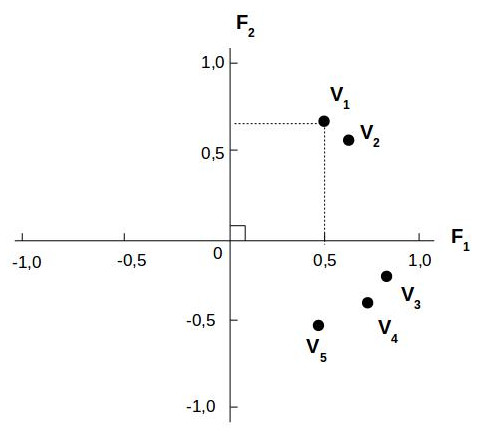
\includegraphics[width=0.8\linewidth,height=\textheight,keepaspectratio]{../../images/AF/fator01.jpg}
\end{column}

\begin{column}{0.48\linewidth}
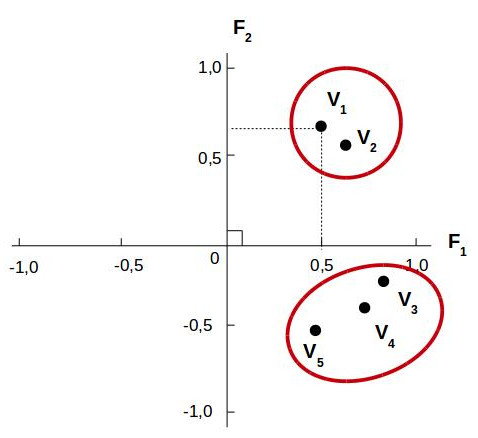
\includegraphics[width=0.8\linewidth,height=\textheight,keepaspectratio]{../../images/AF/fator02.jpg}
\end{column}
\end{columns}
\end{frame}

\begin{frame}{Rotação dos fatores}
\phantomsection\label{rotauxe7uxe3o-dos-fatores-4}
\[\text{Rotação Ortogonal}\]

\begin{columns}[T]
\begin{column}{0.48\linewidth}
\begin{longtable}[]{@{}ccc@{}}
\caption{Cargas fatoriais estimadas para dois
fatores}\label{tbl-fatores2}\tabularnewline
\toprule\noalign{}
Variáveis & Fator 01 & Fator 02 \\
\midrule\noalign{}
\endfirsthead
\toprule\noalign{}
Variáveis & Fator 01 & Fator 02 \\
\midrule\noalign{}
\endhead
\(V_1\) & \(0,03\) & \(0,90\) \\
\(V_2\) & \(0,19\) & \(0,82\) \\
\(V_3\) & \(0,95\) & \(0,22\) \\
\(V_4\) & \(0,89\) & \(0,12\) \\
\(V_5\) & \(0,78\) & \(-0,12\) \\
\bottomrule\noalign{}
\end{longtable}
\end{column}

\begin{column}{0.48\linewidth}
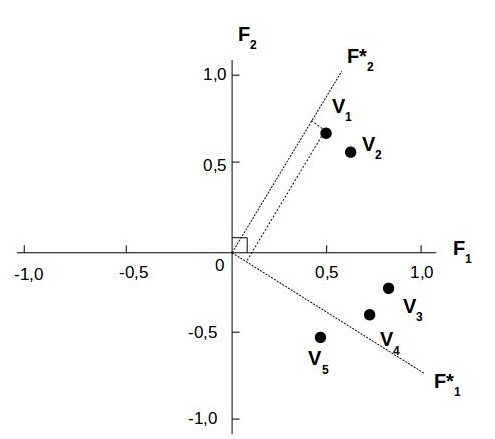
\includegraphics[width=0.8\linewidth,height=\textheight,keepaspectratio]{../../images/AF/fator03.jpg}
\end{column}
\end{columns}
\end{frame}

\begin{frame}{Rotação dos fatores}
\phantomsection\label{rotauxe7uxe3o-dos-fatores-5}
\begin{itemize}
\tightlist
\item
  Os métodos de rotação têm como objetivo simplificar as linhas e
  colunas da matriz fatorial para facilitar a interpretação

  \begin{itemize}
  \tightlist
  \item
    Maximizar a carga de uma variável em um único fator
  \item
    Reduzir ao máximo o número de variáveis com cargas altas por fator
  \end{itemize}
\end{itemize}

\pause

\begin{itemize}
\tightlist
\item
  Alguns critérios para encontrar matriz ortogonal:

  \begin{itemize}
  \tightlist
  \item
    Varimax
  \item
    Quartimax
  \item
    Orthomax
  \end{itemize}
\end{itemize}
\end{frame}

\begin{frame}{Rotação dos fatores}
\phantomsection\label{rotauxe7uxe3o-dos-fatores-6}
\begin{itemize}
\tightlist
\item
  \textbf{Critério Varimax:} É um dos mais utilizados. Em geral, produz
  soluções mais simples
\end{itemize}

\bigskip

\pause

\begin{itemize}
\tightlist
\item
  \textbf{Critério Quartimax:} Tem tendência de gerar fatores, onde
  todas as variáveis têm loadings elevados
\end{itemize}

\bigskip

\pause

\begin{itemize}
\tightlist
\item
  \textbf{Critério Orthomax:} É uma média ponderada dos dois outros
  métodos
\end{itemize}
\end{frame}

\begin{frame}{Rotação dos fatores}
\phantomsection\label{rotauxe7uxe3o-dos-fatores-7}
\begin{block}{Comentários}
\phantomsection\label{comentuxe1rios-1}
\begin{itemize}
\tightlist
\item
  \textbf{Qualidade de ajuste:} A rotação não acrescenta nenhuma
  melhoria em relação ao ajuste original

  \begin{itemize}
  \tightlist
  \item
    Matriz residual original não é alterada pela transformação ortogonal
  \item
    Valores estimados de comunalidade e variâncias específicas
    permanecem inalterados
  \end{itemize}
\end{itemize}

\medskip

\begin{itemize}
\tightlist
\item
  \textbf{Interpretação:} Novos fatores podem ser de mais fácil
  interpretação
\end{itemize}

\medskip

\begin{itemize}
\tightlist
\item
  Quando a solução sem rotação já é de boa qualidade, não se recomenda
  rotação: Solução rotacionada pode ser pior
\end{itemize}
\end{block}
\end{frame}

\begin{frame}{Quantos fatores usar?}
\phantomsection\label{quantos-fatores-usar}
Para determinar o valor de \(m\)\ldots{}

\begin{itemize}
\tightlist
\item
  Analisar a proporção da variação total dos dados atribuída ao
  \(j\)-ésimo fator, dada por:
\end{itemize}

\[\dfrac{\hat{\lambda}_j}{p}, \,\,\,\, j = 1,2, \cdots, m, \text{ se usarmos } \boldsymbol{R}\]

\vspace{0.5cm}

\pause

\begin{itemize}
\tightlist
\item
  \textbf{Critério de Kaiser:} retenção dos fatores com autovalor
  associado superior a 1;
\end{itemize}

\vspace{0.5cm}

\pause

\begin{itemize}
\tightlist
\item
  Gráfico scree-plot
\end{itemize}

\vspace{0.5cm}

\pause

\begin{itemize}
\tightlist
\item
  Análise paralela de Horn
\end{itemize}
\end{frame}

\begin{frame}{Quantos fatores usar?}
\phantomsection\label{quantos-fatores-usar-1}
\begin{itemize}
\tightlist
\item
  Conjugar indicadores estatísticos a:

  \begin{itemize}
  \tightlist
  \item
    Interpretação prática dos resultados;
  \item
    Busca de uma solução parcimoniosa;
  \item
    Possível indicação do número de fatores segundo a teoria da área;
  \end{itemize}
\end{itemize}

\vspace{0.3cm}

\pause

\begin{itemize}
\tightlist
\item
  \textbf{Bom senso (sempre!)}.
\end{itemize}
\end{frame}

\begin{frame}{Quantos fatores usar?}
\phantomsection\label{quantos-fatores-usar-2}
\begin{block}{Comentários}
\phantomsection\label{comentuxe1rios-2}
\begin{itemize}
\tightlist
\item
  \textbf{Método de máxima verossimilhança:} Mudança de valor de \(m\)
  altera as estimativas dos loadings
\end{itemize}

\vspace{0.5cm}

\begin{itemize}
\tightlist
\item
  \textbf{Método de componentes principais:} Aumento no valor de \(m\)
  não altera os loadings para os fatores obtidos anteriormente
\end{itemize}

\vspace{0.5cm}

\begin{itemize}
\tightlist
\item
  Quando os dados provêm de distribuição normal multivariada

  \begin{itemize}
  \tightlist
  \item
    Usar método de componentes principais como análise exploratória dos
    fatores e estimação do valor provável de \(m\)
  \item
    Posteriormente, qualidade da solução inicial poderá ser melhorada
    pelo uso do método de máxima verossimilhança
  \end{itemize}
\end{itemize}
\end{block}
\end{frame}

\begin{frame}{Interpretação dos fatores}
\phantomsection\label{interpretauxe7uxe3o-dos-fatores}
\[\text{Avaliação da significância estatística baseada no tamanho da amostra}\]

\begin{longtable}[]{@{}cc@{}}
\caption{Tamanho mínimo de amostra recomendado em função da carga
fatorial}\tabularnewline
\toprule\noalign{}
Carga Fatorial & Tamanho da amostra \\
\midrule\noalign{}
\endfirsthead
\toprule\noalign{}
Carga Fatorial & Tamanho da amostra \\
\midrule\noalign{}
\endhead
0,30 & 350 \\
0,35 & 250 \\
0,40 & 200 \\
0,45 & 150 \\
0,50 & 120 \\
0,55 & 100 \\
0,60 & 85 \\
0,65 & 70 \\
0,70 & 60 \\
0,75 & 50 \\
\bottomrule\noalign{}
\end{longtable}
\end{frame}




\end{document}
